\begin{frame}[fragile]{measuring round-trip time (1a)}
\begin{Verbatim}[fontsize=\fontsize{10}{11}]
charles@reisst14$ ping 1.1.1.1
PING 1.1.1.1 (1.1.1.1) 56(84) bytes of data.
64 bytes from 1.1.1.1: icmp_seq=1 ttl=52 time=13.8 ms
64 bytes from 1.1.1.1: icmp_seq=2 ttl=52 time=15.0 ms
64 bytes from 1.1.1.1: icmp_seq=3 ttl=52 time=12.5 ms
64 bytes from 1.1.1.1: icmp_seq=4 ttl=52 time=12.3 ms
64 bytes from 1.1.1.1: icmp_seq=5 ttl=52 time=13.5 ms
64 bytes from 1.1.1.1: icmp_seq=6 ttl=52 time=12.5 ms
64 bytes from 1.1.1.1: icmp_seq=7 ttl=52 time=13.3 ms
64 bytes from 1.1.1.1: icmp_seq=8 ttl=52 time=13.2 ms
64 bytes from 1.1.1.1: icmp_seq=9 ttl=52 time=13.3 ms
64 bytes from 1.1.1.1: icmp_seq=10 ttl=52 time=14.1 ms
^C
--- 1.1.1.1 ping statistics ---
10 packets transmitted, 10 received, 0% packet loss, time 9014ms
rtt min/avg/max/mdev = 12.273/13.343/15.024/0.786 ms
\end{Verbatim}
\end{frame}

\begin{frame}[fragile]{measuring round-trip-time (1b)}
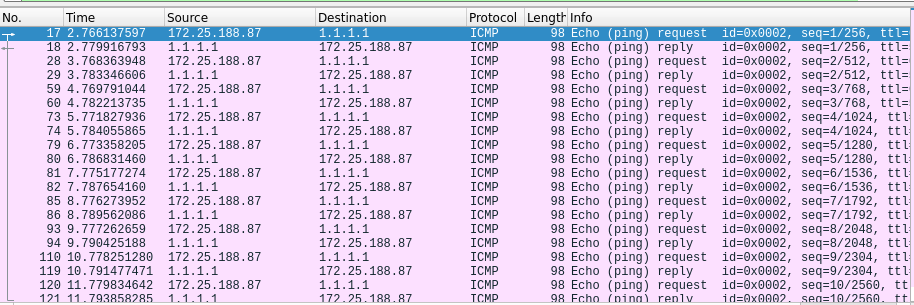
\includegraphics[width=\textwidth]{../perf/icmp-ping-pkts}
\end{frame}

\begin{frame}[fragile]{measuring round-trip-time (1c)}
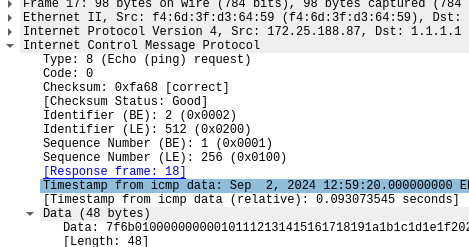
\includegraphics[width=\textwidth]{../perf/icmp-ping-pkt-example}
\end{frame}

\begin{frame}[fragile]{non-ICMP pings (1)}
\begin{Verbatim}[fontsize=\fontsize{10}{11}]
HPING www (enp0s31f6 128.143.67.8): NO FLAGS are set, 40 headers + 0 data bytes                          
len=46 ip=128.143.67.8 ttl=63 DF id=0 sport=0 flags=RA seq=0 win=0 rtt=3.5 ms                            
len=46 ip=128.143.67.8 ttl=63 DF id=0 sport=0 flags=RA seq=1 win=0 rtt=3.2 ms                            
len=46 ip=128.143.67.8 ttl=63 DF id=0 sport=0 flags=RA seq=2 win=0 rtt=7.1 ms                            
len=46 ip=128.143.67.8 ttl=63 DF id=0 sport=0 flags=RA seq=3 win=0 rtt=6.8 ms                            
len=46 ip=128.143.67.8 ttl=63 DF id=0 sport=0 flags=RA seq=4 win=0 rtt=6.5 ms                            
len=46 ip=128.143.67.8 ttl=63 DF id=0 sport=0 flags=RA seq=5 win=0 rtt=6.2 ms                            
len=46 ip=128.143.67.8 ttl=63 DF id=0 sport=0 flags=RA seq=6 win=0 rtt=5.8 ms                            
len=46 ip=128.143.67.8 ttl=63 DF id=0 sport=0 flags=RA seq=7 win=0 rtt=5.4 ms                            
len=46 ip=128.143.67.8 ttl=63 DF id=0 sport=0 flags=RA seq=8 win=0 rtt=5.0 ms                            
len=46 ip=128.143.67.8 ttl=63 DF id=0 sport=0 flags=RA seq=9 win=0 rtt=4.7 ms                            
^C                                                                                                       
--- www hping statistic ---                                                                              
10 packets transmitted, 10 packets received, 0% packet loss                                              
round-trip min/avg/max = 3.2/5.4/7.1 ms
\end{Verbatim}
\end{frame}

\begin{frame}[fragile]{non-ICMP pings (2)}
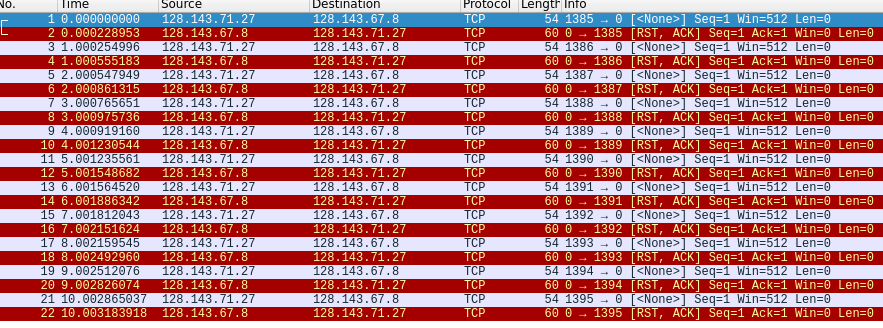
\includegraphics[width=\textwidth]{../perf/hping-wireshark}
\end{frame}

\begin{frame}[fragile]{measuring throughput?}
\begin{Verbatim}[fontsize=\fontsize{10}{11}]
$ scp test.dat portal.cs.virginia.edu:test.dat
test.dat                         100%   32MB  23.0MB/s   00:01    
$ scp portal.cs.virginia.edu:test.dat .
test.dat                         100%   32MB  28.2MB/s   00:01   
\end{Verbatim}
\begin{itemize}
\item (but might be measuring disk speed instead)
\vspace{.5cm}
\item also more specialized tools like \texttt{iperf}
    \begin{itemize}
    \item require program to run on both ends
    \end{itemize}
\end{itemize}
\end{frame}

\begin{frame}[fragile]{measuring throughput}
\begin{Verbatim}[fontsize=\fontsize{10}{11}]
$ iperf -s
------------------------------------------------------------
Server listening on TCP port 5001
TCP window size:  128 KByte (default)
------------------------------------------------------------
[  1] local 128.143.71.87 port 5001 connected with 128.143.71.27 port 54760
[ ID] Interval       Transfer     Bandwidth
[  1] 0.0000-10.0147 sec  1.09 GBytes   934 Mbits/sec
\end{Verbatim}
---
\begin{Verbatim}[fontsize=\fontsize{10}{11}]
$ iperf -c kytos02 | tee iperf.out
------------------------------------------------------------
Client connecting to kytos02, TCP port 5001
TCP window size: 85.0 KByte (default)
------------------------------------------------------------
[  1] local 128.143.71.27 port 54760 connected with 128.143.71.87 port 5001
[ ID] Interval       Transfer     Bandwidth
[  1] 0.0000-10.0256 sec  1.09 GBytes   933 Mbits/sec
\end{Verbatim}
\end{frame}

\begin{frame}[fragile]{measuring transmission delay?}
\begin{Verbatim}[fontsize=\fontsize{10}{11}]
PING www.cs.virginia.edu (128.143.67.8) 1400(1428) bytes of data.
--- www.cs.virginia.edu ping statistics ---
1000 packets transmitted, 1000 received, 0% packet loss, time 50638ms
rtt min/avg/max/mdev = 0.319/0.461/1.222/0.039 ms
$ ping -s 16 www -i 0.05 -c 1000 -q
PING www.cs.virginia.edu (128.143.67.8) 16(44) bytes of data.
--- www.cs.virginia.edu ping statistics ---
1000 packets transmitted, 1000 received, 0% packet loss, time 50995ms
rtt min/avg/max/mdev = 0.156/0.345/1.539/0.068 ms
\end{Verbatim}
\begin{itemize}
\item approx. $0.461 - 0.345 = 0.116$ ms delay for $1400-16$ extra bytes
    \begin{itemize}
    \item with two links in each direction = approx $\frac{0.116}{4}=0.029$ ms/link
    \item $\frac{1400-16 \text{byte}}{0.029 \text{ms}} \approx 50$ Mbit/sec
    \item probably other processing time besides sending on links, though
    \end{itemize}
\end{itemize}
\end{frame}
